\documentclass{article}

% Präambel
%---| Packages |----------------------------------------------------------------

\usepackage{amsmath}    % Create equations and mathematical expressions.
\usepackage{graphicx}   % Embed captioned figures, images and other graphics.
\usepackage{subcaption} % Display images side-by-side.
\usepackage{setspace}   % Custom spacing for TOC entries.
\usepackage[            % Additional citation options.
    backend = biber,
    style   = ieee
]{biblatex}
\usepackage{hyperref}   % Create Links display URLs.
%---| Settings |----------------------------------------------------------------

% Abbildungen
\graphicspath{{./images}}

% Titelseite
\title{Hello world in LaTeX}
\date{\today}
\author{Henry Behrend}

% The setcounter command can be used to set the TOC's depth to to the following
% values (level meaning everything up to the specified section will be shown):
%   0 - nothing
%   1 - section level
%   2 - subsection level
%   3 - subsubsection level (default)
%   4 - paragraph level
%   5 - subparagraph level

% Inhaltsverzeichnis
\setcounter{tocdepth}{3}

% Quellenverzeichnis
\bibliography{sources}

% Links und URLs
\hypersetup{
    pdfborder  = 0 0 0, % Disable the ugly border around links.
    colorlinks = true,
    linkcolor  = black,
    urlcolor   = blue
}

% Round numbers to two decimal places.
\sisetup{
    round-mode      = places,
    round-precision = 2
}

% For backward compatibility.
\pgfplotsset{compat = 1.18}
%---| Commands |----------------------------------------------------------------

% Personally I use the convention that custom defined commands are Pascal case.
\newcommand{\HelloWorld}{\textbf{Hello, world!}}

% Adds parentheses around a footnote reference for better readability.
\renewcommand*{\thefootnote}{(\arabic{footnote})}

\begin{document}

\pagenumbering{gobble}  % This disables page numbering.
\doublespacing          % This increases spacing between lines.

% Titelseite
\maketitle
\newpage

% Inhaltsverzeichnis
\tableofcontents
\newpage

% Abbildungsverzeichnis
\listoffigures
\newpage

% Tabellenverzeichnis
\listoftables
\newpage

\pagenumbering{arabic}
\singlespacing

% Hauptteil
\section{Section}

\HelloWorld

\subsection{Subsection}

Structuring a document is easy!

\subsubsection{Subsubsection}

Here's some text...

\paragraph{Paragraph}

... and here's some more text ...

\subparagraph{Subparagraph}

... and here's even more text!

\section{Some math and equations}

\paragraph{Enumbered equation}

A normal equation with the \texttt{equation} environment:

\begin{equation}
    1 + 2 = 3
\end{equation}

\paragraph{Unenumbered equation}

An unnumbered equation with the \texttt{equation*} environment:

\begin{equation*}
    1 + 2 = 3
\end{equation*}

\paragraph{Multiline equation}

A multiline equation with alignment can be done with the \texttt{align*}
environment:

\begin{align*}
    1 + 2 &= 3 \\
    1 &= 3 - 2
\end{align*}

\paragraph{Complex equations}

More complex equations can be done with commands like \texttt{frac} for
fractions or \texttt{int} for integrals:

\begin{align*}
    f(x) &= x^2 \\
    g(x) &= \frac{1}{x} \\
    F(x) &= \int^a_b \frac{1}{3}x^3
\end{align*}

These commands may be combined into nested equations such as:

\begin{equation*}
    \frac{1}{\sqrt{x}}
\end{equation*}

\paragraph{Matrices}

Displaying matrices is also possible via the \texttt{matrix} environment,
although only within the above mentioned math environments:

\begin{equation*}
    \begin{matrix}
        1 & 0 \\
        0 & 1
    \end{matrix}
\end{equation*}

If there is a need to surround a matrix with brackets, merely wrapping the
\texttt{matrix} command with bracket characters won't do the trick:

\begin{equation*}
    [
        \begin{matrix}
            1 & 0 \\
            0 & 1
        \end{matrix}
    ]
\end{equation*}

Fortunately, there is a way to scale these brackets up to match the height of
the matrix and, for that matter, other equations too:
This can be done by preceeding the opening and closing bracket or parenthesis by
the \texttt{left} and \texttt{right} command respectively.

\begin{equation*}
    \left[
        \begin{matrix}
            1 & 0 \\
            0 & 1
        \end{matrix}
    \right]
\end{equation*}

\begin{equation*}
    \left(\frac{1}{\sqrt{x}}\right)
\end{equation*}

\newpage
\section{Captioned figures and images}

Embedding captioned images and figures into your document by using the
\texttt{figure} environment from the \texttt{graphicx} package:

% The image placement can be controlled by setting the float parameter to one of
% the following values:
%   h (here)     - location in code equals location in the document
%   t (top)      - top of the page
%   b (bottom)   - bottom of the page
%   p (page)     - on a separate page
%   ! (override) - force the specified location (analogous to !important in CSS)
%
% Even stricter placement can be achieved by using the float package's H option.

\begin{figure}[h!]
    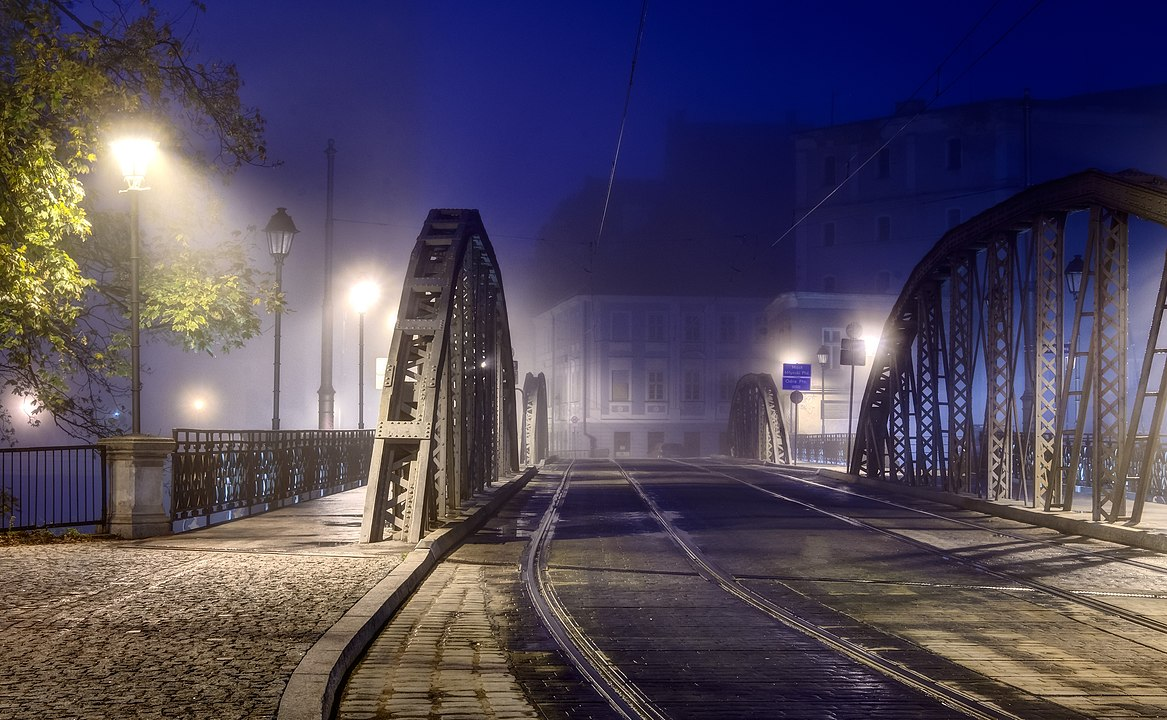
\includegraphics[width=\linewidth]{bridge.jpg}
    \caption{A Bridge.}
    \label{fig:bridge}
\end{figure}

% Most of this paragraph was taken from https://latex-tutorial.com.
Figure \ref{fig:bridge} shows the Mlynski Bridge in Wroclaw. Sometimes when
writing a document, adding single images is not optimal, especially when the
reader is supposed to compare several results or graphs. In such situations, it
might be necessary to use a different environment, called subfigure. The
\texttt{subfigure} environment allows you to place multiple images at a certain
location next to each other and the usage is pretty straightforward:

\begin{figure}[h!]
    \centering
    \begin{subfigure}[b]{0.4\linewidth}
        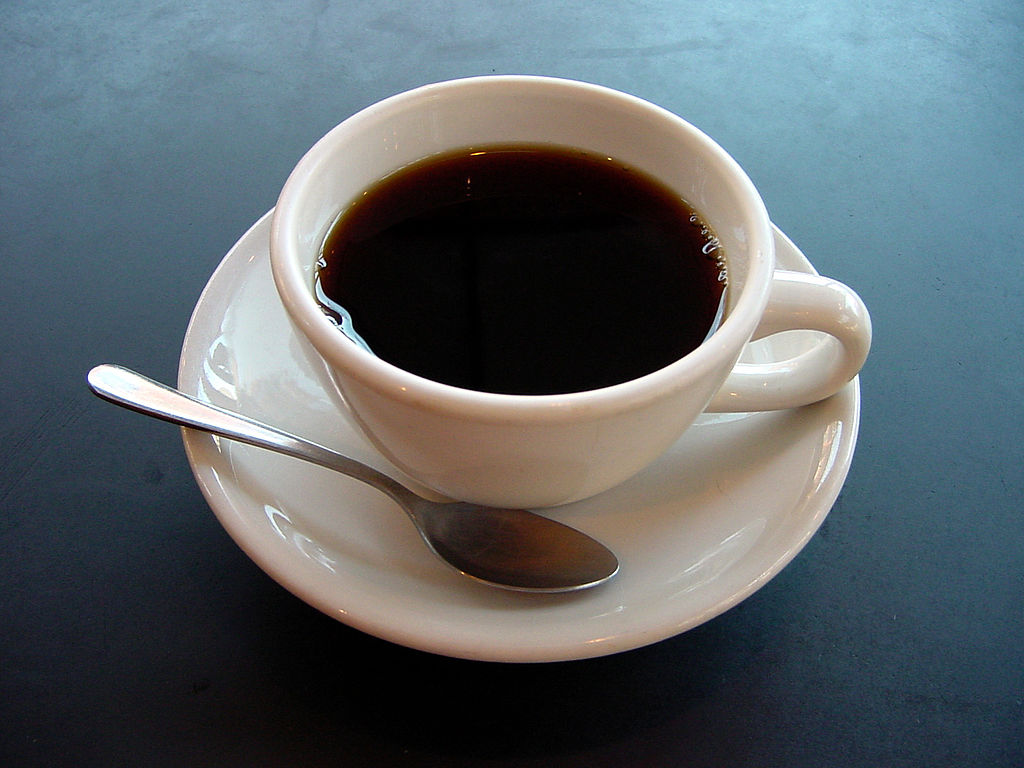
\includegraphics[width=\linewidth]{coffee.jpg}
        \caption{A cup of coffee.}
    \end{subfigure}
    \begin{subfigure}[b]{0.4\linewidth}
        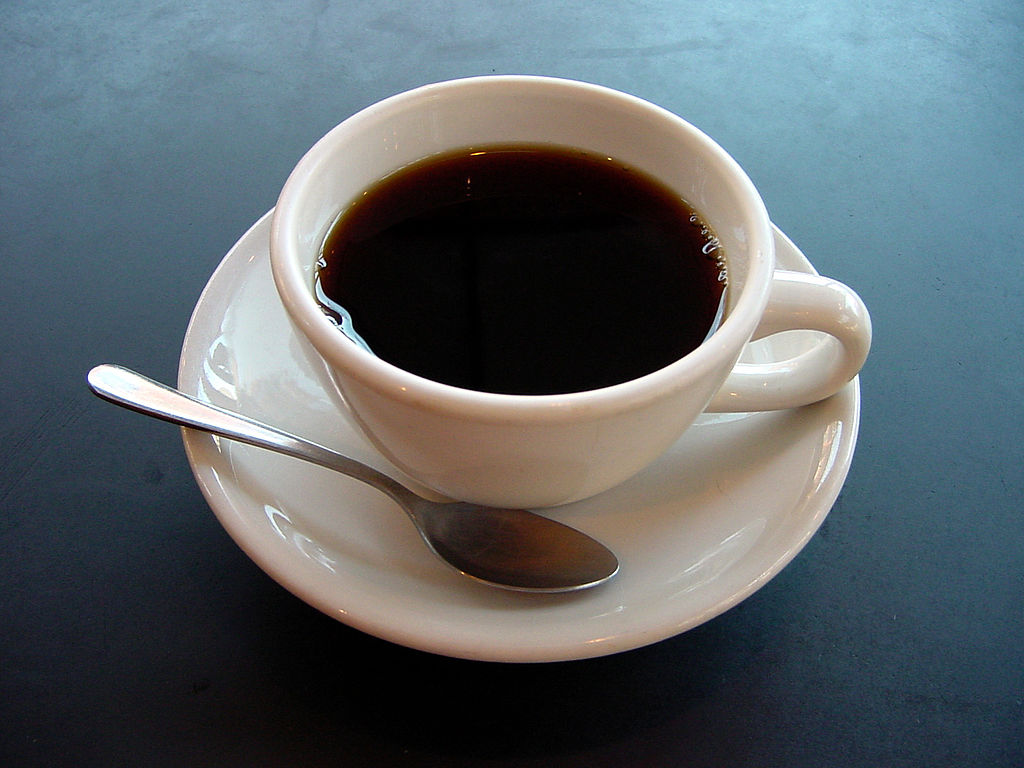
\includegraphics[width=\linewidth]{coffee.jpg}
        \caption{Another cup of coffee.}
    \end{subfigure}
    \caption{Two cups of coffee side by side.}
    \label{fig:coffee}
\end{figure}

\section{Table of contents (TOC)}

The TOC can be generated automatically via the \texttt{tableofcontents} command.
By default, sections, subsections and subsubsections are displayed there, this
called the TOC's depth. The depth can be changed via the \texttt{setcounter}
command by setting its first argument to \texttt{tocdepth} and the second
argument to the desired value.

It is also possible to set the depth locally rather than for the whole document
by calling the \texttt{addtocontents} command before declaring the sections to
be affected by the local depth setting. An example can be seen right below:

\addtocontents{toc}{\setcounter{tocdepth}{1}}

\section{A section with a custom depth value for the TOC}

The following subsection and subsubsection should not be part of the TOC.

\subsection{I'm not part of the TOC}

\subsubsection{Me neither}

% This resets the TOC's depth value, since 3 is the default.
\addtocontents{toc}{\setcounter{tocdepth}{3}}

\section{A new section with the global depth value}

\subsection{I'm in the TOC again!}

\section{Bibliography and citations}

Managing sources and citations is really easy with \LaTeX. There are external
tools for creating and maintaining bibliographies, like \textit{Biblatex} or
\textit{Bibtex} in case of this particular project.

\subsection{Creating the bibliography}

The bibliography is created by calling the \texttt{bibliography} command and the
preferred citation style is set via the \texttt{bibliographystyle} command.
Bibtex requires the creation of a \texttt{.bib} file, which holds the
bibliographic information. To see how such a file is structured, take a look at
the file \texttt{bibliography.bib} located in the project's root folder.

\subsection{Citation}

After setting up the bibliography, the \texttt{cite} command is used to cite,
refer or quote the source material contained in the bibliography. A really good
book for example would be \autocite{mindstorms}.

\subsection{Biblatex}

Although Biblatex is quite good for the above mentioned use cases, it is limited
to basic citation styles. If citing literature in footnotes is necessary for
example, Biblatex isn't really helpful for that kind of task and should be
swapped in favor of a more versatile alternative like Biblatex. Biblatex can
and will be used here on top of Bibtex and thus extends its the feature set. It
has to be made available first by incuding the \texttt{biblatex} package. Then,
the used \texttt{.bib} file has to be specified with the \texttt{bibliography}
command inside the preamble. Creating the bibliography is done via the
\texttt{printbibliography} command where we created the bibliography before.
Additonally, citations are created by calling \texttt{autocite} instead of
\texttt{cite}.

Footnotes can be created by either setting the \texttt{style} package option to
\texttt{verbose-trad2} or any other citation style which includes footnotes for
that matter. All available values for the \texttt{style} can be found \href{https://ctan.joethei.xyz/macros/latex/contrib/biblatex/doc/biblatex.pdf#subsection.3.3}{here}.

% Quellenverzeichnis
\newpage
\printbibliography

\end{document}